% ----------------------------------------------------------------------------------------
%--- CHAPTER INTRODUCTION ----------------------------------------------------------------
% ----------------------------------------------------------------------------------------
\chapter{Introduction} \label{introduction}

\enquote{\emph{Pantha Rhei}} is, according to \emph{Plato}, one of the famous
philosophical statements first described by the Greek philosopher
\emph{Heraclitus}\footnote{\url{https://plato.stanford.edu/entries/process-philosophy/}}.
Translated as \enquote{everything flows} this statement is an unambiguous commitment to
ubiquitous dynamics of everything that exists. \enquote{Life is flux}, one of the
constants in life is change.

In the realms of Software Engineering, the \enquote{laws of software evolution}
\parencite[]{lehman_programs_1980} refers to a series of laws described by
\citeauthor{lehman_programs_1980}. With these Laws, he describes the balance between the
forces driving new developments on the one hand (a change) and the forces that slow down
progress on the other hand. Based on \emph{Heraclitus} philosophical statement, we know
software engineering projects will frequently be subjected to change, probably due to
changing functional requirements and technological progress. As these changes emerge, the
complexity of these projects will gradually increase over time due to the increasing
number of combinatorial effects. Eventually, this will render the system obsolete,
according to \citeauthor{lehman_programs_1980} \parencite[]{lehman_programs_1980}.

As the competitive environments of contemporary organizations are changing continuously,
the speed at which changes emerge is also increasing. IT organizations are
attempting to cope with this trend by adopting agility and maturing their agile practices
\parencite[]{2024_SIM_key_issues_and_trends}. Therefore, agility has been defined as a measure for
contemporary organizations to adapt to new environments and cope with rapid change
\parencite[]{neumann_strategic_1994}.

% ----------------------------------------------------------------------------------------
%--- SECTION INTRODUCING SOFTWARE EVOLVABILITY -------------------------------------------
% ----------------------------------------------------------------------------------------
\section{Introducing Software evolvability}
the effort to apply change should stay constant over time, regardless of the type of change,
whether it would be a functional, technical or architectural change.

<<To-do: Link software evolvability to the first part of the introduction>>\\
<<To-do: Link combinatorial effects to a measure to determine software evolvability>>

% ----------------------------------------------------------------------------------------
%--- SECTION INTRODUCING NORMALIZED SYSTEMS THEOREMS -------------------------------------
% ----------------------------------------------------------------------------------------
\section{Introducing Normalized Systems Theorems}
<<To-do: Link normalized systems as a measure to create software evolvability>>

% ----------------------------------------------------------------------------------------
%--- SECTION INTRODUCING CLEAN ARCHITECTURE ___-------------------------------------------
% ----------------------------------------------------------------------------------------
\section{Introducing Clean Architecture}
<<To-do: Link normalized systems as a measure to create software evolvability>>

% ----------------------------------------------------------------------------------------
%--- SECTION PROBLEM STATEMENT -----------------------------------------------------------
% ----------------------------------------------------------------------------------------
\section{Problem statement} \label{problem_statement} 

Since the introduction of Normalized Systems Theorems, Java EE (Java Enterprise Edition)
was used as a programming language in scientific research settings to describe the
evolvability of software architectures based on the stability concepts of systems theory
\parencite[]{mannaert_towards_2012}. \citeauthor{mannaert_towards_2012} stated in the
paper that the design theorems were formulated as modular structures that are independent
of any software language or development paradigm.

Java EE is still a prevalent programming language for enterprise- and IT organizations.
Many software solutions are created and maintained using this programming language.

% ----------------------------------------------------------------------------------------
%--- SECTION HYPOTHESIS -----------------------------------------------------------
% ----------------------------------------------------------------------------------------
\section{Hypothesis} \label{hypothesis}
1. explain that NS already has been a proven theory
    - and that it mitigates combinatorial effects
    - improving software evolvability
    - prescribed design of emerging elements based on principles
2. theorize that CA does a similar thing and has the same effect on the design
3. theorize that NS is also applicable for C\# artifacts.

\begin{figure}[!h]
    \centering
    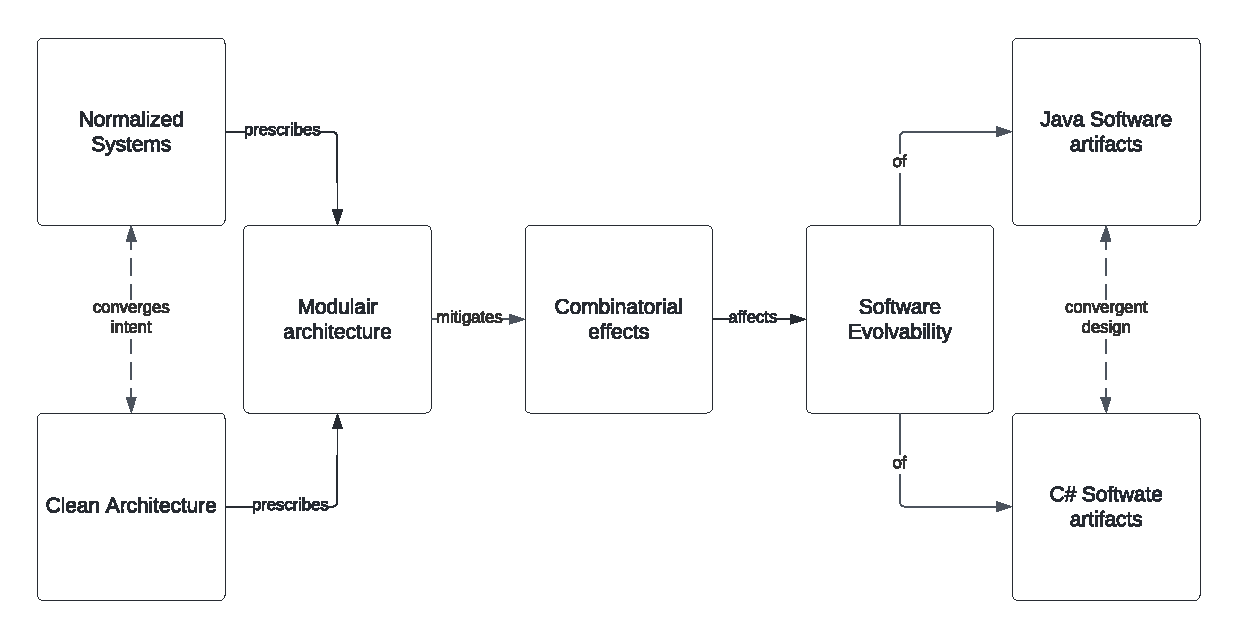
\includegraphics[width=1\textwidth]{Figures/hypothesis.pdf}
    \caption[The hypothesis graphically.]{The hypothesis graphically.}
    \label{fig:hypothesis}
\end{figure}

% ----------------------------------------------------------------------------------------
%--- SECTION RESEARCH SUBJECT -----------------------------------------------------------
% ----------------------------------------------------------------------------------------
\section{Conceptual framework} \label{conceptual_framework}
Figure \ref{fig:overall_conceptual_framework} depicts the conceptual research framework.
It describes the hypothesis that Normalized Systems Theorems have a positive impact on the
total amount of combinatorial effects on C\# based information systems.

\begin{figure}[!h]
    \centering
    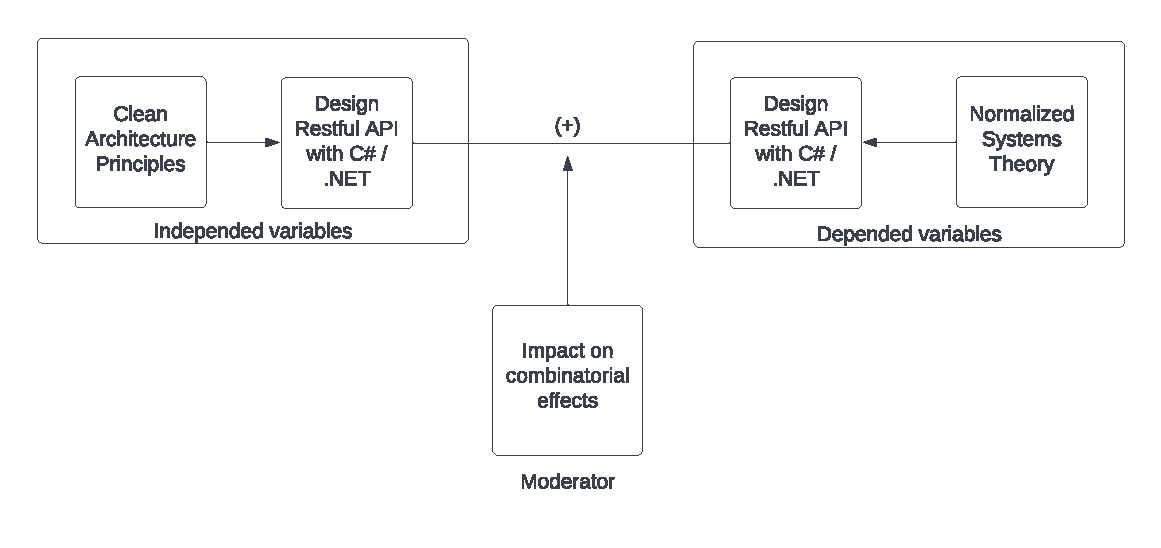
\includegraphics[width=1\textwidth]{Figures/overall_conceptual_framework}
    \caption[Overall conceptual framework]{Overall conceptual framework.}
    \label{fig:overall_conceptual_framework}
\end{figure}
\newpage
% ----------------------------------------------------------------------------------------
%--- SECTION RESEARCH QUESTION -------------------------------------------------------------------
% ----------------------------------------------------------------------------------------
\section{Research questions} \label{research_questions}
Considering the hypothesis described in \ref{conceptual_framework} the following research
is determined:

\begin{center}
    \enquote*{\textit{What is the applicability of Normalized Systems Theorems
    on restful API's designed based on the Clean Architecture principles and build with
    C\#/.NET}}
\end{center}

The following sub-questions can be formulated that support the research on the main
research question:
\begin{itemize}
    \item What is the literature stating about evolvable software systems.
    \item What is the literature stating about combinatorial effects on software changes in software systems.
    \item What is the literature stating on how one can measure combinatorial effects of a change on a software system.
    \item Which principles of Clean Architecture contribute to a reduction of
    combinatorial effects, in a way that they complement the theorems of normalized
    systems.
\end{itemize}